\section{Experiments}

\subsection{Machine Specification}
We executed the following tests using this environment:

%TODO Please Bera write down your machine spec.

\begin{itemize}
    \item \textbf{Machine}:
    \begin{itemize}
        \item Type: HP OmniBook Ultra Flip 14
        \item CPU: Intel® Core™ Ultra 7 - 258V (4.8 GHz, 12 MB cache L3, 8 core, 8 thread)
        \item RAM: 32 GB LPDDR5x-8533 MT/s
    \end{itemize}
    \item \textbf{Software}:
    \begin{itemize}
        \item OS: Ubuntu 24.04.3 LTS (Noble Numbat) x86\_64
        \item Host: Windows Subsystem for Linux - Ubuntu (2.5.7.0)
        \item Kubernetes: minikube version: v1.36.0, configured with 4 cores and 16GB of RAM
    \end{itemize}
\end{itemize}

\subsection{Experiments Description}
The experiments have the goal of emulating different types of traffic, with the objective of showing the system behavior. The possible experiments can be performed choosing different rates following a state machine. In other words, if the user selects 4 different rates for the distribution selected the load is composed of 4 circularly executed states with the rated specified. The duration of each state is editable from the code.

So, for example, choosing a uniform distribution with all rates value such that min=max (to model the deterministic arrival process) and selecting a test with a duration of 9 minutes and rates = ([1,1];[2,2];[3,3];[5,5]) we are modelling an arrival process that generates a load with 1 message/s for 1 minute, than 2 messages/s for 1 minute, than 3 messages/s for 1 minute, than 5 messages/s for 1 minute. At this point 4 minutes has been passed so the arrival process restarts circularly from 1 message/s and so on until the end of the test.

\subsection{Experiments guide}
In this section we include a miniguide to reproduce our experiments. First of all it is necessary to clone the GitHub repository at \href{https://github.com/Berags/oris-predictive-autoscaler}{this link} (https://github.com/Berags/oris-predictive-autoscaler). To start the project is necessary, as a minimum dependancy, to have installed \href{https://minikube.sigs.k8s.io/docs/}{Minikube}. After having installed successfully Minikube, execute the following command:

\begin{table}[!htb]
\centering
\begin{tabular}{c}
\begin{lstlisting}
minikube start
\end{lstlisting}
\end{tabular}
\end{table}

then, it is sufficient to position the terminal on the directory of the project where it is present the .sh file named ./start.sh and execute:

\begin{table}[!htb]
\centering
\begin{tabular}{c}
\begin{lstlisting}
./start.sh
\end{lstlisting}
\end{tabular}
\end{table}
the file start.sh contains all the instruction necessary to build and run our project (i.e. all the containers and components). Don't mind if it takes a while, it is perfectly normal due to the project complexity. At this point, as reported in \guillemotleft port-forward.sh\guillemotright \ you can monitor:
\begin{itemize}
  \item The RabbitMQ queue at \guillemotleft http://localhost:15672\guillemotright
  \item Prometheus at \guillemotleft http://localhost:9090\guillemotright
  \item Grafana (with all the dashboards of interest shown below) at \guillemotleft http://localhost:3000\guillemotright, the default username and password is \verb|admin|.
  \item Kafdrop (for the Kafka queue) at \guillemotleft http://localhost:9000\guillemotright
\end{itemize}

At this point everything is ready to start the tests. In order to do it, go ( we suggest with an additional terminal window) in the folder of \guillemotleft build-and-run.sh\guillemotright \ that is inside the \guillemotleft k6 \guillemotright folder and execute the file with
\begin{table}[!htb]
\centering
\begin{tabular}{c}
\begin{lstlisting}
./build-and-run.sh
\end{lstlisting}
\end{tabular}
\end{table}

\begin{lstlisting}[mathescape]
1. Exponential
2. Poisson ($\lambda$<100)
3. Uniform (Use min = max for deterministic)
4. Erlang (k, $\lambda$)
5. Exit
----------------------------
Insert your choice:
\end{lstlisting}

In this way in the console is shown the test menu from which you can choose the distribution of the load you want to simulate. The available distributions are the above. Then, remains only to choose the rates as described before and how you can see below. Then, the test starts and the console reports some logs. To monitor the entire system consult the addresses above. 

\subsubsection{Experiment personalization}

Copying the repository you can essentially modify the code as you prefer but if you want to modify the transition time is sufficient to modify the following instruction:

\begin{table}[!htb]
\centering
\begin{tabular}{c}
\begin{lstlisting}
const transitionTime = DistributionFactory.getDeterministic(60);
\end{lstlisting}
\end{tabular}
\end{table}

in rabbitmq-test.js and with \guillemotleft 60\guillemotright \ that are the seconds of permanence in each state. If you are not interested in a deterministic transition you can substitute it, for example, with an Exponential one with:

\begin{table}[!htb]
\centering
\begin{tabular}{c}
\begin{lstlisting}
const transitionTime = DistributionFactory.getExponential(20);
\end{lstlisting}
\end{tabular}
\end{table}


Please notice ho we modeled arrival processes of our interest using the js library included in the code repo under k6/lib (all the documentation inside), but eventually you can use also the others distributions supported.

\subsubsection{Setup Details}

If you are wondering what are the uses of others \textit{.sh} files, this is the right section. Essentially, the fundamental ones are \guillemotleft start.sh\guillemotright \ and \guillemotleft build-and-run.sh\guillemotright \ but since ./start.sh does a lot of work and when something goes wrong is not everytime necessary to rebuild everything, we provided \guillemotleft port-forward.sh\guillemotright \ for the port forwarding only and \guillemotleft delete\_and\_deploy\_sirio.sh\guillemotright \ to, as its name suggests, delete and redeploy only sirio.

\subsection{Arrival Modeling}
For all the test, we modeled in Sirio the Arrival process as an Exponential with parameter $\lambda$ equal to the inverse of the average inter-arrival time of the messages in the queue (or $\lambda$ equals to the average messages per second, it's the same). 

We also tried using Bernstein phase types, but we encountered a problem that stopped it. It seems that the Sirio model of a Bernstein phase type uses a rapidly increasing amount of RAM while increases the number of phases. For instance, we tried 50 phases and the scaler tried to instance in the heap more than 768MB, making the pods overflow and be killed by Kubernetes. With a lower number of phases, we didn't achieve a good enough approximation to be used in the scaler. In the other hand, trying to extend the amount of RAM available to the Sirio pod make the machine's OS trashing most of the time.

In addition to that, we found the approximation with the exponential more that capable to a uniform arrival rate. Then, having a microservice controller that consumes so much resource seem odd and counterproductive.

\subsection{Rejection Rate Calculation}
Here we want to discuss how we calculated the rejection rate, and the reasons to choose it. For our experiments, we wanted to calculate a relative rejection rate. In fact, we consider this approach more robust if compared to an absolute rejection rate target.

The rejection rate, at least in terms of expected value, can be defined as: \textit{the probability that a packed get rejected by the queue}. To verify this condition, two pre-conditions must be true:
\begin{itemize}
    \item The Queue is full.
    \item The arrival process is habilitated to push a new message.
    \item The arrival process extracts a time to fire smaller than the service process.
\end{itemize}

Considering a stochastic model expressed in term of a Stochastic Time Petri Net (STPN), we are interested in only three elements: the place of the queue, the last transition of the arrival process that goes into the queue, and the first transition of the service that pulls from the queue (most of the time the service is represented with only a transition). For this problem we assume that the stochastic properties of the model depends only on the marking state. So, let $R$ be the event of a rejection, $Q=q_{max}$ the event of a marking with the queue full, $A$ the event of a marking where the last arrival transition has a token as a precondition, $t_a$ and $t_s$ the values sampled from the arrival and service transitions, and $\lambda_a$ and $\lambda_s$ the arrival and service rate respectively, from the previous conditions we can derive the equation \ref{eq:rejection}:

\begin{equation}
    \label{eq:rejection}
    \begin{split}        
    P(R)& =P(Q=q_{max} \land A\land t_a<t_s)\\
    & = P(t_a<t_s|Q=q_{max})P(Q=q_{max} \land A)
    \end{split}
\end{equation}

Considering that we used a Markovian model, the arrival and service transitions samples their times to fire form exponential transitions. So, let $\lambda_a$ and $\lambda_s$ of two transition when the queue is full, we can rewrite equation \ref{eq:rejection} as \ref{eq:rejection_exp}:
\begin{equation}
    \label{eq:rejection_exp}
    \begin{split}
    P(R) & =  P(t_a<t_s|Q=q_{max}\land A)P(Q=q_{max}\land A) \\
     & = P(Exp(\lambda_a)<Exp(\lambda_s))P(Q=q_{max}\land A)
    \end{split}
\end{equation}

Can be easily derived the probability of an exponential samples before another as in equation \ref{eq:first_exp}, the final rejection rate formula it \ref{eq:rejection_fin}.
\begin{gather}
P(Exp(\lambda_a)<Exp(\lambda_s)) = \frac{\lambda_a}{\lambda_a + \lambda_s} \label{eq:first_exp}\\
P(R)=\frac{\lambda_a}{\lambda_a + \lambda_s}P(Q=q_{max}\land A) \label{eq:rejection_fin}
\end{gather}

Considering that given a closed model Sirio is capable to enumerate all the reachable states, using the steady state analysis we can get the probability of having a state where the queue is full and the arrival transition is enable, while using the \textit{MarkingExpresions} getting transition rates is trivial.

Here below, to highlight how this formula can be translated in practice, is reported the code that calculated the rejection rate.
\begin{lstlisting}
BigDecimal rejection = BigDecimal.ZERO;
Map<Marking, BigDecimal> results = RegSteadyState.builder().build().compute(pn, m).getSteadyState();
for (Marking tmp : results.keySet()) {
    if (tmp.getTokens(queuePlace) == queue.getSize() && pn.isEnabled(arrivalTransition, tmp)) {
        BigDecimal currentRejection = results.get(tmp);

        BigDecimal arrivalRate = extractLambda(arrivalTransition, tmp).setScale(8, RoundingMode.HALF_UP);
        BigDecimal serviceRate = extractLambda(serviceTransition, tmp).setScale(8, RoundingMode.HALF_UP);

        currentRejection = currentRejection.multiply(arrivalRate).divide(arrivalRate.add(serviceRate), 8, RoundingMode.HALF_DOWN);

        rejection = rejection.add(currentRejection);
    }
}
return rejection;
\end{lstlisting}

\subsection{Experiments Setup}
In all tests we set some common parameters:
\begin{enumerate}
    \item Rejection Rate: 5\%.
    \item Service Rate: 1.
    \item Duration of states in the arrival process: 60s.
    \item Total test duration: 20 minutes.
\end{enumerate}

For the experiments with constant arrival time, we defined a state machine with the following parameters: [0.33,0.33],[0.2,0.2],[0.11,0.11],[1,1],[0.14,0.14]. In this, for every state we sample the same inter arrival time with the following expected messages per second: 3, 5, 9, 1 and 7. Considering that the state machine is cyclic, this behavior repeats periodically.

On the other hand, we tried a stochastic workload using exponential as inter arrival time distributions in the machine states. The parameters used are: 3, 5, 7, 1, 9. These are also the expected messages per second of the respectively state.

In this report, we separated the logic of establishing the optimal number of replicas (the Recommender) from the one that communicates with Kubernetes (Updater). This allows to apply different scaling logics to the workers. In the following we will confront an immediate application of the recommendation, versus a sliding window approach that waits a series of downscale recommendation before applying it.

\subsection{Results}
\subsubsection{Immediate Apply of Recommendations}

In executing this experiment, both for constant and exponential arrival rates, we measure the arrived and rejected messages in figures \ref{fig:default_constant_messages} and \ref{fig:default_exponential_messages}.

\begin{figure}[H]
	\begin{subfigure}{0.49\linewidth}
	    \centering
	    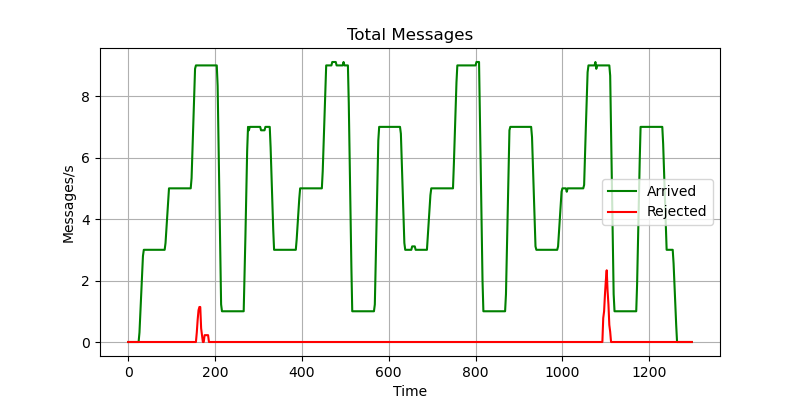
\includegraphics[width=1\linewidth]{images/default/constant/messages.png}
	    \caption{Arrived and Rejected messages per second in constant rates.}
	    \label{fig:default_constant_messages}
	\end{subfigure}
	\begin{subfigure}{0.49\linewidth}
	    \centering
    		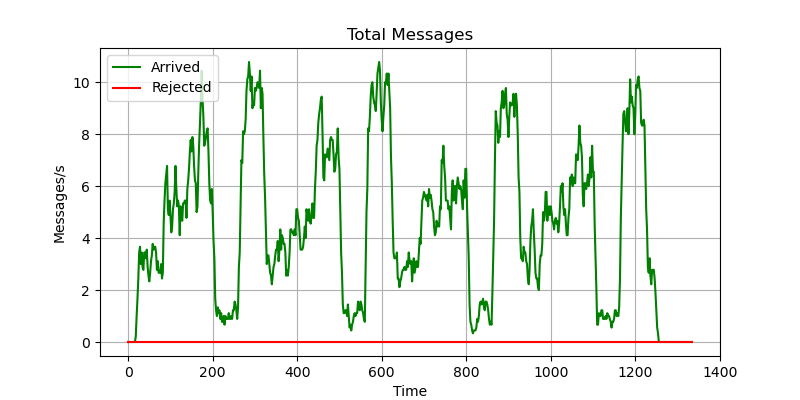
\includegraphics[width=1\linewidth]{images/default/exponential/messages.png}
	    \caption{Arrived and Rejected messages per second with exponential arrival times.}
    		\label{fig:default_exponential_messages}
	\end{subfigure}
	\begin{subfigure}{0.49\linewidth}
	    \centering
	    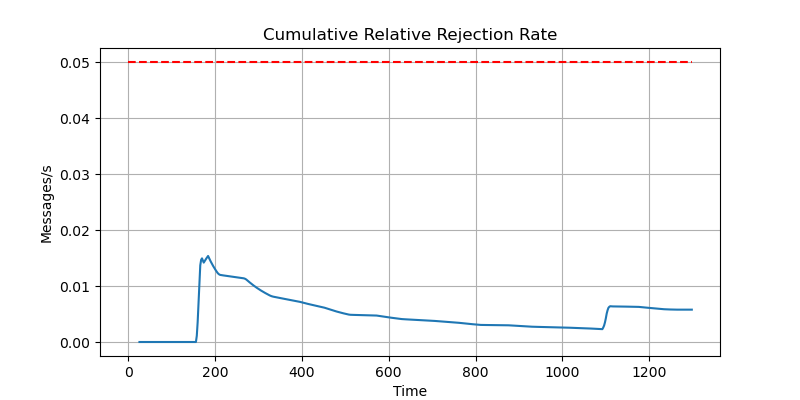
\includegraphics[width=1\linewidth]{images/default/constant/rejection_cumulative.png}
	    \caption{Cumulative Rejection rate for constant arrival time experiment.}
	    \label{fig:default_constant_rejection}
	\end{subfigure}
	\begin{subfigure}{0.49\linewidth}
	    \centering
	    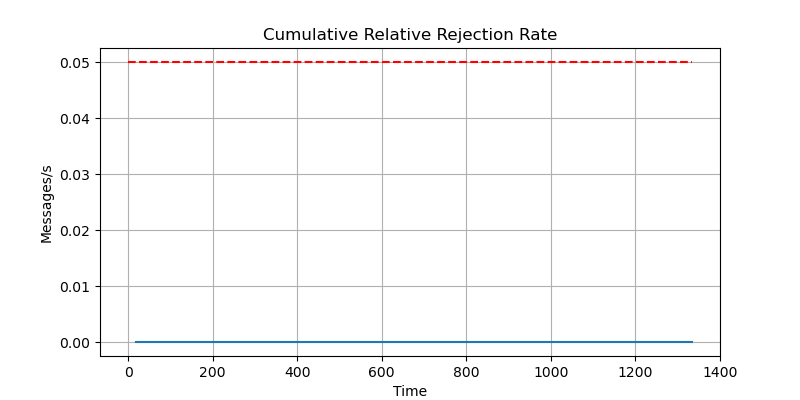
\includegraphics[width=1\linewidth]{images/default/exponential/rejection_cumulative.png}
	    \caption{Cumulative Rejection rate for exponential arrival time experiment.}
	    \label{fig:default_exponential_rejection}
	\end{subfigure}
\end{figure}

As said, the goal of the control is to keep a rejection rate below 5\%. For both of them, rejection rate was under the threshold, with even the exponential without rejected messages at all.

We wanted to see not only if the target was achieved, but also the evolution in the number of recommended pods. The trend of the scaling can be seen in figures \ref{fig:default_constant_pods} and \ref{fig:default_exponential_pods}, with the respective lag cost in figures \ref{fig:default_constant_lag} and \ref{fig:default_exponential_lag}. More detail on how the cal cost is calculated can be found in section \ref{sec:lag_cost}.

\begin{figure}[H]
	\begin{subfigure}{0.49\linewidth}
	    \centering
	    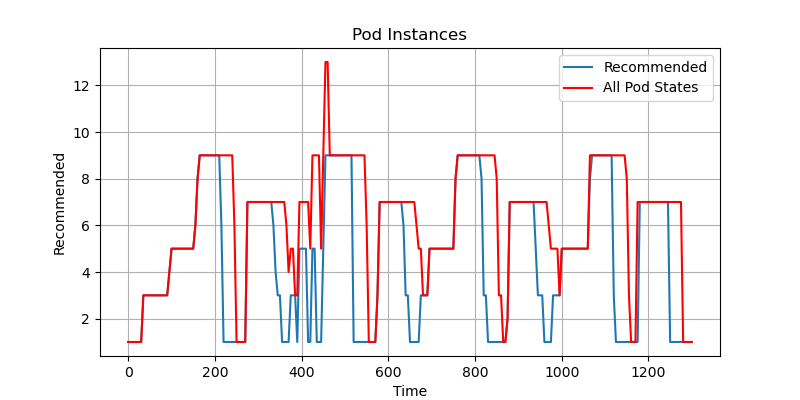
\includegraphics[width=1\linewidth]{images/default/constant/pods.png}
	    \caption{Number of pods trend for constant arrival time experiment.}
	    \label{fig:default_constant_pods}
	\end{subfigure}
	\begin{subfigure}{0.49\linewidth}
	    \centering
    		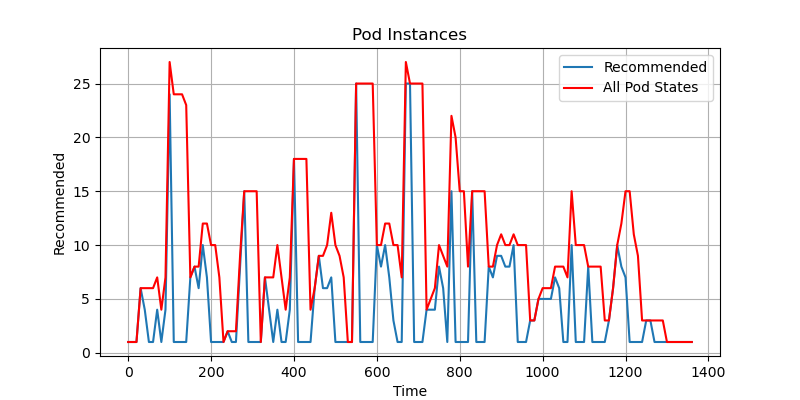
\includegraphics[width=1\linewidth]{images/default/exponential/pods.png}
	    \caption{Number of pods trend for exponential arrival time experiment.}
    		\label{fig:default_exponential_pods}
	\end{subfigure}
	\begin{subfigure}{0.49\linewidth}
	    \centering
	    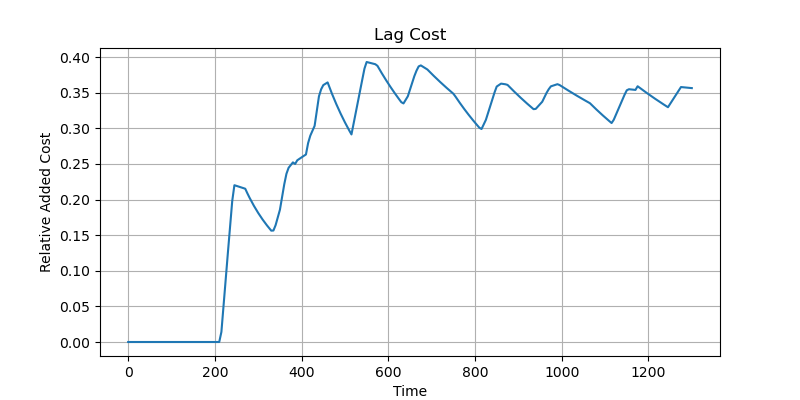
\includegraphics[width=1\linewidth]{images/default/constant/lag_cost_cumulative.png}
	    \caption{Cumulative lag cost for constant arrival time experiment.}
	    \label{fig:default_constant_lag}
	\end{subfigure}
	\begin{subfigure}{0.49\linewidth}
	    \centering
	    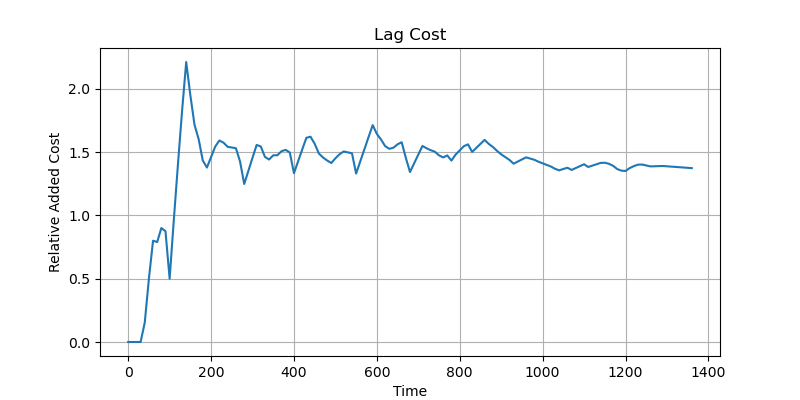
\includegraphics[width=1\linewidth]{images/default/exponential/lag_cost_cumulative.png}
	    \caption{Cumulative lag cost for exponential arrival time experiment.}
	    \label{fig:default_exponential_lag}
	\end{subfigure}
\end{figure}

The surge of lag cost came mainly from downscaling. In fact, we the Sirio Scaler recommend to scale up the pods Kubernetes immediately starts creating them to match the the new incoming traffic. On the other hand, when Sirio recommend a downscale the surplus pods cannot be terminated instantaneously, mainly because these pods are still elaborating some elements.

Another issue that make lag cost spike is that pods can be much higher than the recommendation. This appends when recommendation drops and rise very shortly. In fact, the first drop make most of the pods terminating, but when the second rise comes, given that terminating pods cannot be recovered, we need to instantiate even more to compensate.

A summary of this results can be seen in table \ref{tab:default_summary}.

\begin{table}[h]
	\centering
	\begin{tabular}{|c|c|c|}
		\hline
		& Constant & Exponential \\
		\hline
		Recommended Cost & 6030 & 2880 \\
		\hline
		Effective Cost & 8180 & 6835 \\
		\hline
		Relative Lag & 35.66\% & 137.33\%  \\
		\hline
		Rejection Rate & 0.58\% & 0.00\% \\
		\hline
	\end{tabular}
	\caption{Summary of the results for the immediate application of recommendations.}
	\label{tab:default_summary}
\end{table}

\subsubsection{Sliding Window}
In our experimenting we also tired to implement an updater that uses a sliding window to reduce the lag cost. In the case of a recommendation to increase the number of pods that will be immediately implemented, in the case of a reduction the system maintains some inertia before doing it.

More precisely, for every downscaling the recommended value is inserted into a history. When the history reaches a certain dimension, and this history has values smaller of the current value the target is updated with the maximum in the history. Every time the target is changed the history is cleared.

For more details, below there is the snipped of code that implements this behavior.

\begin{lstlisting}
int currentReplicas = getCurrentReplicas();

if (newReplicas > currentReplicas) {
	replicaHistory.clear(); 
	return newReplicas;
} else if (newReplicas < currentReplicas) {
	replicaHistory.add(newReplicas);
	if (replicaHistory.size() > scalingDecisionWindow) {
		replicaHistory.removeFirst();	
	}

	if (replicaHistory.size() >= scalingDecisionWindow
         && replicaHistory.stream().allMatch(r -> r <= currentReplicas)) {                
		int maxInHistory = replicaHistory.stream().max(Integer::compareTo).orElse(newReplicas);
		replicaHistory.clear();
		return maxInHistory;
	}
} else {
	replicaHistory.add(newReplicas);
}
return currentReplicas;
\end{lstlisting}

As in the precedent couple of test, in the following we report the trend of arrived messages confronted with the cumulative rejection rate.

\begin{figure}[H]
	\begin{subfigure}{0.49\linewidth}
	    \centering
	    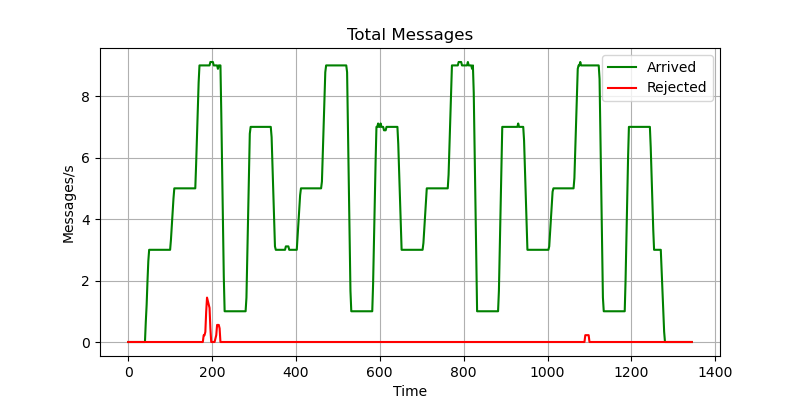
\includegraphics[width=1\linewidth]{images/sliding_window/constant/messages.png}
	    \caption{Arrived and Rejected messages per second in constant rates.}
	    \label{fig:sliding_window_constant_messages}
	\end{subfigure}
	\begin{subfigure}{0.49\linewidth}
	    \centering
    		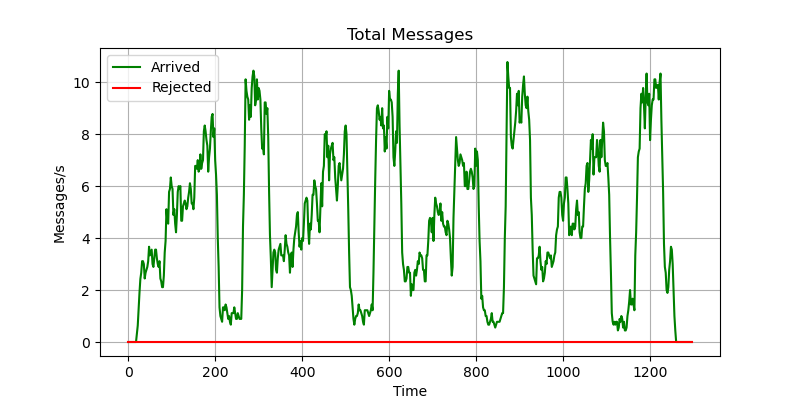
\includegraphics[width=1\linewidth]{images/sliding_window/exponential/messages.png}
	    \caption{Arrived and Rejected messages per second with exponential arrival times.}
    		\label{fig:sliding_window_exponential_messages}
	\end{subfigure}
	\begin{subfigure}{0.49\linewidth}
	    \centering
	    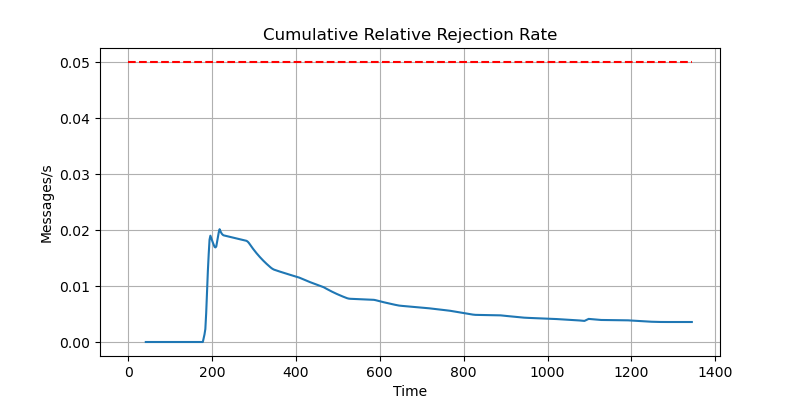
\includegraphics[width=1\linewidth]{images/sliding_window/constant/rejection_cumulative.png}
	    \caption{Cumulative Rejection rate for constant arrival time experiment.}
	    \label{fig:sliding_window_constant_rejection}
	\end{subfigure}
	\begin{subfigure}{0.49\linewidth}
	    \centering
	    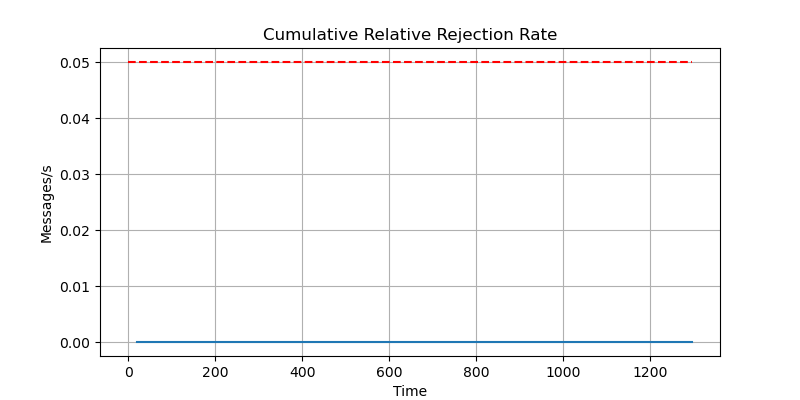
\includegraphics[width=1\linewidth]{images/sliding_window/exponential/rejection_cumulative.png}
	    \caption{Cumulative Rejection rate for exponential arrival time experiment.}
	    \label{fig:sliding_window_exponential_rejection}
	\end{subfigure}
\end{figure}

In the same way, the following figures shows the recommended pods with the associated cumulative lag cost.

\begin{figure}[H]
	\begin{subfigure}{0.49\linewidth}
	    \centering
	    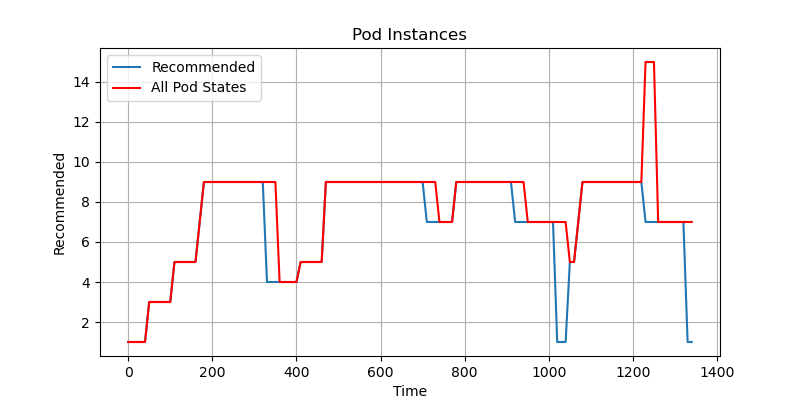
\includegraphics[width=1\linewidth]{images/sliding_window/constant/pods.png}
	    \caption{Number of pods trend for constant arrival time experiment.}
	    \label{fig:sliding_window_constant_pods}
	\end{subfigure}
	\begin{subfigure}{0.49\linewidth}
	    \centering
    		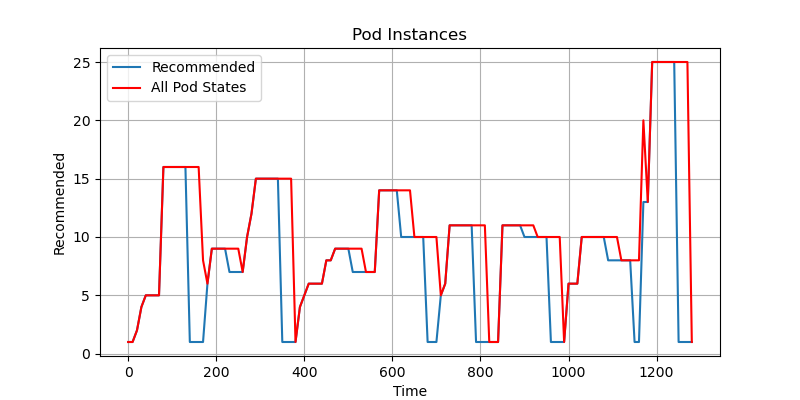
\includegraphics[width=1\linewidth]{images/sliding_window/exponential/pods.png}
	    \caption{Number of pods trend for exponential arrival time experiment.}
    		\label{fig:sliding_window_exponential_pods}
	\end{subfigure}
	\begin{subfigure}{0.49\linewidth}
	    \centering
	    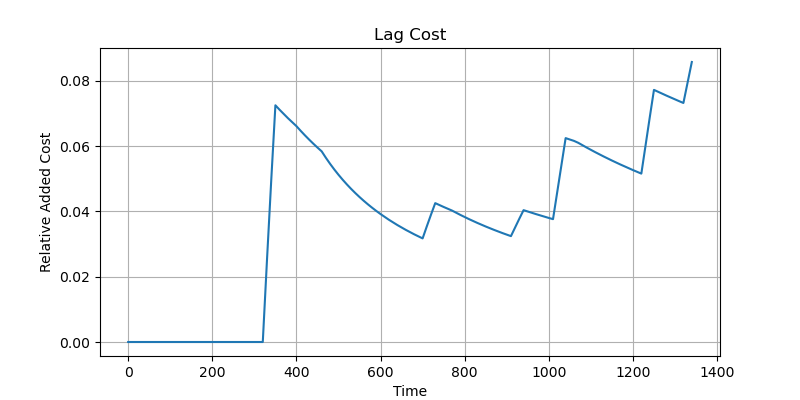
\includegraphics[width=1\linewidth]{images/sliding_window/constant/lag_cost_cumulative.png}
	    \caption{Cumulative lag cost for constant arrival time experiment.}
	    \label{fig:sliding_window_constant_lag}
	\end{subfigure}
	\begin{subfigure}{0.49\linewidth}
	    \centering
	    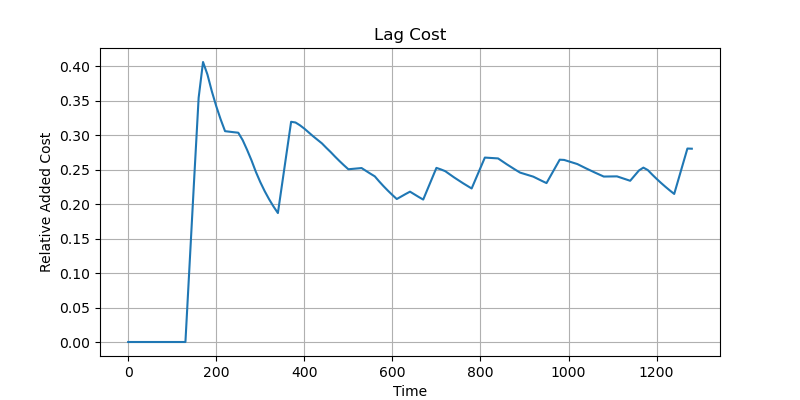
\includegraphics[width=1\linewidth]{images/sliding_window/exponential/lag_cost_cumulative.png}
	    \caption{Cumulative lag cost for exponential arrival time experiment.}
	    \label{fig:sliding_window_exponential_lag}
	\end{subfigure}
\end{figure}

Lastly, table \ref{tab:sliding_window_summary} report a summary of experiments using the sliding window approach.

\begin{table}[h]
	\centering
	\begin{tabular}{|c|c|c|}
		\hline
		& Constant & Exponential \\
		\hline
		Recommended Cost & 4725 & 5420 \\
		\hline
		Effective Cost & 5130 & 6940 \\
		\hline
		Relative Lag & 8.57\% & 28.04\%  \\
		\hline
		Rejection Rate & 0.36\% & 0.00\% \\
		\hline
	\end{tabular}
	\caption{Summary of the results for the sliding window approach.}
	\label{tab:sliding_window_summary}
\end{table}

\subsubsection{Comments}
From the above result many thing can be observed. Before commenting them, it's important to notice that the total amount of messages generated in every case is mostly the same.

The first result that can we notice is that, introducing a sliding window reduces significantly the cost introduced by Kubernetes lag. However, this reduction is mostly due to a rising in the recommended cost. In fact, in the case of a constant arrival time we have got a lower total cost, but in the case of the exponential not a significant change (in reality a slight increase, but that can explained by run-to-run variations).

Certainly the sliding window strategy made the number of pods more stable during time, avoiding excessive peak usage of resources. To better frame this concept, in previous experiments in a different setting and a different machine the exponential case without sliding window always crashed, while using it allowed for a termination without issued.

Another interesting trend that can be seen in this data is that, for some reason, the constant inter arrival time seems harder to manage that the exponential. In both cases the constant arrival rate is characterize by some rejected messages, while the exponential no. For this phenomenon we can't say if it happened by chance of if there is some hidden reason.

Lastly. something can be said in reference to the very low recommended number cost achieved (in theory) in the exponential case without sliding window. We can see how it's very common see it going to 1. Due to the fact that both the arrival and service processes are stochastic, can happen that the queue goes empty. This makes the CDF generator component of the system fail to generate valid CDF. If Sirio doesn't receive any messages for a give time (10s) simply \textit{thinks} that there is not more load, and recommend for the minimum amount of pods (1 in this case). It's important to notice that terminating pods are probably still elaborating at least the last messages that they were able to pull, factually discharging the queue. These two phenomenon combined make possible to achieve very low recommended cost, but still a 0 rejection rate. The effective cost metric catches this behavior.

